
\documentclass[a4paper,12pt]{article}
\usepackage{amsmath, amssymb}
\usepackage{xcolor}
\usepackage{tcolorbox}
\usepackage{multicol}
\usepackage{geometry}
\graphicspath{ {../Images/} }
\hyphenpenalty=100000

\geometry{left=1.5cm, right=1.5cm, top=2cm, bottom=2cm}

\tcbuselibrary{theorems}

\definecolor{PurpleEx}{HTML}{5d478b}
\definecolor{GrayEx}{HTML}{f2f2f2}
\definecolor{GrayBG}{HTML}{d9d9d9}
\definecolor{BlackSav}{HTML}{000000}

\title{
\centering
\tcbset{colframe=BlackSav,colback=GrayBG}
\tcbox[tikznode]{
Chapitre 1 \\ Polynômes du second degré 
}
}
\usepackage{tikz}
\author{}
\date{}

\newtcbtheorem
  []% init options
  {exercice}% name
  {Exercice}% title
  {%
    colback=GrayEx,
    colframe=PurpleEx,
    fonttitle=\bfseries,
  }% options
  {ex}% prefix


\begin{document}

\maketitle

\begin{multicols}{2}

\begin{exercice}[title=Exercice 1 \quad$\star$\quad\  {[Calculer]}]{}{}
Calculer le déterminant de chaque polynôme ci-dessous.
\begin{enumerate}
    \item \(3x^2 + 2x + 1\)
    \item \(2x^2 - 2x - 4\)
    \item \(-3x^2 + 2x - 5\)
    \item \(x^2 + x + 1\)
    \item \(x^2 - 7\)
    \item \(x - x^2 + 3\)
    \item \(7x - 3 + x^2\)
    \item \(1 - 3x^2\)
\end{enumerate}
\end{exercice}

\begin{exercice}[title=Exercice 2 \quad$\star$\quad\  {Calculer}]{}{}
Déterminer la forme factorisée, lorsqu’elle existe, des polynômes suivants.
\begin{enumerate}
    \item \(x^2 + 3x - 4\)
    \item \(2x^2 - 4x - 12\)
    \item \(-3x^2 + x - 5\)
    \item \(x^2 + x + 1\)
    \item \(x^2 - 2x + 1\)
    \item \(-4x^2 + 2\)
\end{enumerate}
\end{exercice}

\begin{exercice}[title=Exercice 3 \quad$\star$\quad\ {[Calculer]}]{}{}
Résoudre dans \( \mathbb{R} \) les équations suivantes.
\begin{enumerate}
    \item \(x^2 + 4 = 0\)
    \item \(3x^2 - x - 6 = 0\)
    \item \(x^2 - 10x + 25 = 0\)
    \item \(x^2 - 3x + 3 = 0\)
    \item \(x^2 - 1 = 0\)
    \item \(x - 4x^2 + 7 = 0\)
\end{enumerate}
\end{exercice}

\begin{exercice}[title=Exercice 4 \quad$\star$\quad\  {[Calculer]}]{}{}
Déterminer les racines des polynômes suivants.
\begin{enumerate}
    \item \(x^2 - x - 1\)
    \item \(x^2 - x\)
    \item \(-5x^2 + 7x + 12\)
    \item \(-3x - x^2 + 4\)
    \item \(3x^2 - 6x + 3\)
    \item \(-x + x^2 + 7\)
\end{enumerate}
\end{exercice}

\begin{exercice}[title=Exercice 5 \quad$\star\star$\quad\ {[Calculer, Raisonner]}]{}{}
Soit \(m \in \mathbb{R}\). On considère l'équation \(x^2 - mx + m + 2 = 0\). Pour quelles valeurs de \(m\) l'équation admet-elle une unique solution ?
\end{exercice}

\begin{exercice}[title=Exercice 6 \quad$\star\star$\quad\ {[Calculer, Modéliser]}]{}{}
Déterminer deux entiers naturels consécutifs dont le produit est égal à 64262.
\end{exercice}

\begin{exercice}[title=Exercice 7 \quad$\star$\quad\  {[Calculer]}]{}{}
Les équations suivantes admettent toutes des racines. Dans chaque cas, déterminer le produit et la somme des racines.
\begin{enumerate}
    \item \(x^2 - x - 2\)
    \item \(x^2 - \pi x\)
    \item \(-x^2 + 3x + 12\)
    \item \(3x + x^2 - 1\)
    \item \(\sqrt{17}x^2 + 32x - 1\)
    \item \(2x - 3x^2 + 5\)
\end{enumerate}
\end{exercice}

\begin{exercice}[title=Exercice 8 \quad$\star\star$\quad\  {[Calculer]}]{}{}
Déterminer deux réels \(x_1\) et \(x_2\) vérifiant les conditions suivantes :
\begin{equation*}
\begin{cases}
x_1 + x_2 = 5 \\
x_1 x_2 = 1
\end{cases}
\end{equation*}
\end{exercice}

\begin{exercice}[title=Exercice 9 \quad$\star\star$\quad\  {[Calculer]}]{}{}
Existe-t-il des réels \(a\) et \(b\) vérifiant les conditions suivantes ?
\begin{equation*}
\begin{cases}
a + b = -3 \\
ab = 2
\end{cases}
\end{equation*}
Si oui, déterminer lesquels.
\end{exercice}

% ... continue adding exercises following the same format ...
% Suite des exercices après l'exercice 9
\begin{exercice}[title=Exercice 10 \quad$\star\star$\quad\  {[Calculer]}]{}{}
Existe-t-il des réels \(a\) et \(b\) vérifiant les conditions suivantes ?
\begin{equation*}
\begin{cases}
a + b = 4 \\
ab = 5
\end{cases}
\end{equation*}
Si oui, déterminer lesquels.
\end{exercice}

\begin{exercice}[title=Exercice 11 \quad$\star\star\star$\quad\ {[Calculer, Chercher]}]{}{}
Soient les réels \(a\) et \(b\) les solutions de l’équation \(2x^2 - 7x + 5 = 0\). Calculer \(a^2 + b^2\).
\end{exercice}

\begin{exercice}[title=Exercice 12 \quad$\star$\quad\ {[Calculer]}]{}{}
Résoudre les équations suivantes en utilisant la méthode la plus adaptée (facteur commun, identité remarquable, calcul avec le discriminant, racine évidente, etc.)
\begin{enumerate}
    \item \(x^2 + 4x = 0\)
    \item \(\sqrt{2}x^2 + 3x - 1 = 0\)
    \item \(\pi x^2 + 2\pi x + \pi = 0\)
    \item \(x^2 + x + 1 = 0\)
    \item \(x^2 - x - 2 = 0\)
    \item \(x^2 + 7 = 0\)
    \item \(x^2 - 12x = -36\)
    \item \(-3x^2 - 1 = 0\)
    \item \(3x^2 + 3x + 0 = 0\)
    \item \(7x^2 + x + 2 = 0\)
    \item \((x - 5)(x + 7) = 0\)
    \item \((x - 3)(x + 1) = 6\)
    \item \(x^2 = \sqrt{2}\)
\end{enumerate}
\end{exercice}

\begin{exercice}[title=Exercice 13 \quad$\star\star$\quad\  {[Calculer]}]{}{}
Déterminer le signe des polynômes suivants.
\begin{enumerate}
    \item \((x - 1)(x - 4)\)
    \item \(5x^2 - x - 1\)
    \item \(x^2 + 3x - 1\)
    \item \(x^2 + x + 4\)
    \item \(-5x^2 + 3x + 11\)
    \item \(x^2 - 8x + 16\)
    \item \(-3x^2 + 8x - 11\)
\end{enumerate}
\end{exercice}

\begin{exercice}[title=Exercice 14 \quad$\star\star$\quad\  {[Calculer]}]{}{}
Résoudre dans \( \mathbb{R} \) les inéquations suivantes.
\begin{enumerate}
    \item \((x - 1)(x + 1) \geq 0\)
    \item \(7x^2 + 3x \leq 0\)
    \item \(2x^2 + x - 1 < 0\)
    \item \(x^2 + x + 5 < 0\)
    \item \(-x^2 + 4x - 4 \leq 0\)
    \item \(-3x^2 + 5x - 1 > 0\)
\end{enumerate}
\end{exercice}

\begin{exercice}[title=Exercice 15 \quad$\star\star\star$\quad\  {[Calculer]}]{}{}
Résoudre dans \( \mathbb{R} \) les inéquations suivantes.
\begin{enumerate}
    \item \(\dfrac{x - 1}{x + 1} \geq x + 3\)
    \item \(\dfrac{x^2 - 2}{x^2+x+1} < 0\)
    \item \(\dfrac{x^2 -2x -5}{x^2 - 3} \leq 0\)
    \item \(\dfrac{x + 1}{2x + 3} \geq -x + 2\)
\end{enumerate}
\end{exercice}

\begin{exercice}[title=Exercice 16 \quad$\star$\quad\  {[Raisonner]}]{}{}
Dans tout l’exercice, \(f\) désigne la fonction définie sur \( \mathbb{R} \) par \( f(x) = ax^2 + bx + c \) (avec \( a \neq 0 \)). Pour chaque affirmation, indiquer si elle est vraie ou fausse. Énoncer par ailleurs sa réciproque et indiquer également si elle est vraie ou fausse.
\begin{enumerate}
    \item Si \(a < 0\), alors pour tout \( x \in \mathbb{R} \), \(f(x) < 0\).
    \item Si deux polynômes du second degré ont même racines, alors ils sont égaux.
\end{enumerate}
\end{exercice}

\begin{exercice}[title=Exercice 17 \quad$\star\star$\quad\ {Raisonner, Communiquer}]{}{}
Soit \(f\) la fonction définie sur \( \mathbb{R} \) par \( f(x) = ax^2 + bx + c \) (avec \( a \neq 0 \) et \( c \neq 0 \)). Montrer que si \(a\) et \(c\) sont de signes contraires, alors \(f\) admet nécessairement deux racines réelles.
\end{exercice}

\begin{exercice}[title=Exercice 18 \quad$\star\star\star$\quad\ {[Calculer, Chercher]}]{}{}
Étudier le signe de la fonction \( f \) définie sur \( \mathbb{R} \) par
\[
f(x) = \dfrac{|x^2 - 2x - 3| - 3}{|x| + 1}.
\]
\end{exercice}

\begin{exercice}[title=Exercice 19 \quad$\star$\quad\  {[Calculer]}]{}{}
Dresser le tableau de variations des fonctions suivantes (définies sur \( \mathbb{R} \)).
\begin{enumerate}
    \item \( f_1(x) = x^2 + 3x + 1 \)
    \item \( f_2(x) = 5x^2 - x - 1 \)
    \item \( f_3(x) = x^2 - x \)
    \item \( f_4(x) = 1 - 2x^2 \)
    \item \( f_5(x) = 7x - 2 \)
    \item \( f_6(x) = -5x^2 + 3x + 7 \)
\end{enumerate}
\end{exercice}

\begin{exercice}[title=Exercice 20 \quad$\star\star$\quad\  {[Calculer]}]{}{}
Dresser le tableau de variations des fonctions suivantes (définies sur \( \mathbb{R} \)).
\begin{enumerate}
    \item \( f_1(x) = \dfrac{-x^2}{3} + \sqrt{2} \)
    \item \( f_2(x) = \dfrac{x^2}{3} - \dfrac{x}{2} - 4 \)
    \item \( f_3(x) = (x - 2)(x - 6) \)
    \item \( f_4(x) = -5(x - 1)(x + 9) \)
    \item \( f_5(x) = -3x^2 - 3x + 2 \)
    \item \( f_6(x) = (x + \sqrt{2})(x - \pi) \)
\end{enumerate}
\end{exercice}

\begin{exercice}[title=Exercice 21 \quad$\star\star$\quad\  {[Calculer]}]{}{}
Résoudre dans \( \mathbb{R} \) les équations de degré trois suivantes.
\begin{enumerate}
    \item \(x^3 + x - 2 = 0\)
    \item \(3x^3 - x + 2 = 0\)
    \item \(x^3 + 5x^2 + x = 0\)
    \item \(x^3 + 3x^2 - 2x = 0\)
    \item \(x^3 - 3x - 2 = 0\)
\end{enumerate}
\end{exercice}

\begin{exercice}[title=Exercice 22 \quad$\star\star$\quad\  {[Calculer]}]{}{}
Résoudre dans \( \mathbb{R} \) les équations bicarrées suivantes.
\begin{enumerate}
    \item \(x^4 + x^2 - 5 = 0\)
    \item \(x^4 - 4x^2 + 2 = 0\)
    \item \(x^4 - 10x^2 + 25 = 0\)
    \item \(x^4 - 3x^2 + 7 = 0\)
    \item \(x^4 - 2 = 0\)
\end{enumerate}
\end{exercice}

\begin{exercice}[title=Exercice 23 \quad$\star\star$\quad\ {[Calculer, Représenter]}]{}{}
Déterminer l’unique fonction \( f \) polynôme du second degré dont la courbe représentative passe par les points \( A(0;5) \), \( B(2;3) \) et \( C(-1;9) \).
\end{exercice}

\begin{exercice}[title=Exercice 24 \quad$\star\star$\quad\ {[Calculer, Représenter]}]{}{}
Déterminer l’unique fonction \( f \) polynôme du second degré dont la courbe représentative passe par les points \( A(0;3) \), \( B(1;7) \) et \( C(-3;5) \).
\end{exercice}

\begin{exercice}[title=Exercice 25 \quad$\star\star\star$\quad\ {[Calculer, Représenter]}]{}{}
Déterminer l’unique fonction \( f \) polynôme du second degré dont la courbe représentative passe par les points \( A(4;1) \), \( B(10;-7) \) et \( C(-2;5) \).
\end{exercice}

\begin{exercice}[title=Exercice 26 \quad$\star\star$\quad\ {Modéliser}]{}{}
Une entreprise agricole produit du lait. Une étude statistique a permis d’estimer que le coût total de production (en €) est modélisé par la fonction \( C \) définie par :
\[
C(x) = 3,54 \cdot 10^{-4} x^2 + 446,298x + 10,53
\]
où \( x \) est le nombre de milliers de litres produit annuellement, \( x \) étant compris entre 0 et 700. L’entreprise vend toute sa production au prix de 446,53 € les 1000 litres. On note \( B(x) \) le bénéfice de l’entreprise, c’est-à-dire la différence entre les recettes et le coût de production, pour la vente de \( x \) milliers de litres de lait.
\begin{enumerate}
    \item Montrer que :
    \[
    B(x) = -3,54 \cdot 10^{-4} x^2 + 0,232x - 10,53.
    \]
    \item Dans quel intervalle doit se situer la production pour que l’activité soit rentable ?
    \item Combien de milliers de litres de lait l’entreprise doit-elle produire afin d’obtenir un bénéfice maximal ?
\end{enumerate}
\end{exercice}

\begin{exercice}[title=Exercice 27 \quad$\star\star$\quad\ {[Modéliser]}]{}{}
Sur route sèche, la distance d’arrêt d’une voiture est donnée par \( D = \dfrac{v^2}{14} + 2v \) où \( v \) est la vitesse de la voiture au début du freinage (exprimée en m.s\(^{-1}\)).
\begin{enumerate}
    \item Si une voiture roule à 130 km.h\(^{-1}\), quel sera la distance d’arrêt (arrondir au mètre près) ?
    \item À quel intervalle doit appartenir la vitesse (en km.h\(^{-1}\)) pour que la distance d’arrêt soit inférieure à 100 m (arrondir à l’unité près) ?
\end{enumerate}
\end{exercice}

\begin{exercice}[title=Exercice 28 \quad$\star\star$\quad\ {[Modéliser, Calculer]}]{}{}
On considère un carré \( ABCD \) de côté 1. \( EFGH \) est un carré tel que :
\begin{itemize}
    \item Les points \( E \), \( F \), \( G \), \( H \) appartiennent respectivement aux côtés \([AB]\), \([BC]\), \([CD]\) et \([AD]\).
    \item \( AE = BF = CG = DH = x \) avec \( 0 \leq x \leq 1 \).
\end{itemize}
\begin{center}
    \hspace{2em}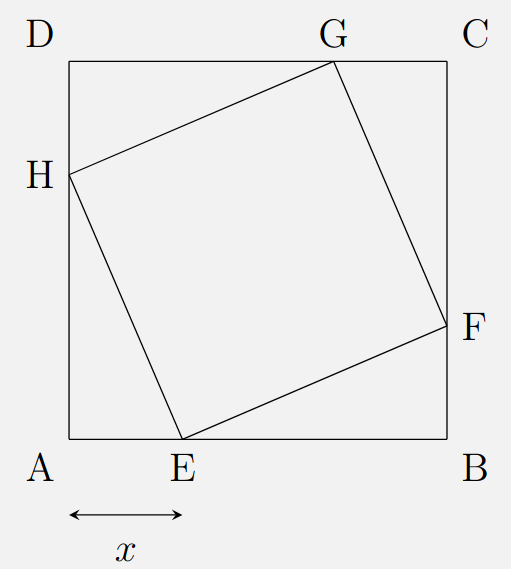
\includegraphics[width=0.7\linewidth]{Screenshot from 2024-11-04 13-17-10.png}
\end{center}
\begin{enumerate}
    \item On note \( A(x) \) l’aire du carré \( EFGH \). Montrer que pour tout \( x \in [0;1] \) :
    \[
    A(x) = 2x^2 - 2x + 1.
    \]
    \item En déduire la valeur de \( x \) pour laquelle l’aire du carré \( EFGH \) est minimale.
\end{enumerate}
\end{exercice}

\begin{exercice}[title=Exercice 29 \quad$\star\star\star$\quad\ {[Calculer, Raisonner]}]{}{}
Résoudre les équations suivantes :
\begin{enumerate}
    \item \(\sqrt{3x + 1} = x\)
    \item \(\sqrt{x - 1} = 2x\)
    \item \(\sqrt{7x/2 + 5} = x - 1\)
    \item \(\sqrt{x^2 + 5x} = 3 \sqrt{x}\)
    \item \(\sqrt{x^2 + x + 1} = 3\sqrt{x}\)
    \item \(\sqrt{x^2 - 2x + 2} = \sqrt{x}\)
\end{enumerate}
\end{exercice}

\begin{exercice}[title=Exercice 30 \quad$\star\star\star$\quad\ {[Calculer, Chercher]}]{}{}
On appelle « nombre d’or » et on note \( \phi \) la solution positive de l’équation \( x^2 = x + 1 \). En utilisant la calculatrice, calculer la valeur exacte de \( \phi^{32} \).
\end{exercice}

\begin{exercice}[title=Exercice 31 \quad$\star\star\star$\quad\ {[Calculer, Chercher, Représenter]}]{}{}
Pour quelles valeurs de \( k \in \mathbb{R}^+ \) existe-t-il un rectangle tel que son aire et son périmètre soient égaux à \( k \) ?
\end{exercice}

\begin{exercice}[title=Exercice 32 \quad$\star\star\star$\quad\ {[Modéliser, Chercher, Calculer]}]{}{}
La distance Terre-Lune est d’environ 384 000 kilomètres. La masse de la Terre est de \(5,97 \times 10^{24}\) kg et celle de la Lune est de \(7,35 \times 10^{22}\) kg. Déterminer en quelle(s) position(s) de l’axe Terre-Lune doit se trouver un astéroïde pour que la force gravitationnelle exercée par la Terre sur l’astéroïde et la force gravitationnelle exercée par la Lune sur l’astéroïde se compensent ?
\end{exercice}

\end{multicols}

\end{document}
